\documentclass[12pt]{article}
%\usepackage{amsfonts}
%\usepackage{amssymb}
%\usepackage{amsmath}
%\usepackage{listings}
%\lstset{language=[LaTeX]TeX}

\begin{document}
\title {The Alignment Toolkit}
\author{Ara V. Nefian \\ Taemin Kim\\
\{ara.nefian,taemin.kim\}@nasa.gov}
\maketitle

This document describes a basic use structure of the AlignmentTK (ATK). ATK is developed for 2D and 3D data alignment and supports the following applications:
\begin{itemize}
\item assembler - aligns two DEMs, to be used in rover localization with a large orbital map. It uses iterative clsoest point (ICP) algorithm and has 
been tested for MER imagery in the context of HiRISE orbital maps.
\item lidar2dem - aligns DEM to lidar data. It uses ICP and has been tested on several DEMs and LOLA tracks.
\item lidar2img - aligns lidar to images. It uses a affine transform to match the LOLA simulated reflectance to Apollo imagery.
\item stereo\_processing - creates 3D point clouds from stereo image pairs
\item sfm\_processing - performs structure from motion on pairs of images
\end{itemize} 

\section{How to install the Alignment Toolkit}
You can simply follow the first subsection to build and test the ATK once you installed its prerequisites such as OpenCV 2.3.1, PCL 1.5, lapack, cmake and gfortran. The complete installation procedure of the prerequisites on the Mac OS X is described in \ref{sec:How to install Prerequisites}.

\subsection{How to build and test the ATK:}
\begin{enumerate}
	\item{svn co  https://babelfish.arc.nasa.gov/svn/stereopipeline/sandbox/lima} - download the ATK
	\item{mkdir lima/build \&\& cd lima/build}
	\item{cmake ..} - here is big double dots 
	\item{make install} - executables are installed in usr/local/bin by default (see the section \ref{sec:How to change BIN directory} to change the location of executables.)
	\item{make test} - view the details in the file lima/build/Testing/Temporary/LastTest.log
\end{enumerate}

\subsection{How to run SFM:}
\begin{enumerate}
	\item{mkdir lima/examples \&\& cd lima/examples}
	\item{Copy images and their depth data with their file lists (e.g., testImageList.txt and testPCList.txt) and configuration file (e.g., testConfig.txt)}
	\item{sfm\_test testConfig.txt testImageList.txt results} - where testImageList.txt contains the list of input images
	* make sure the bin directory is in \$PATH.
\end{enumerate}

\subsection{How to install Prerequisites:}\label{sec:How to install Prerequisites}

\begin{enumerate}
	\item{} install Macport (http://www.macports.org/install.php) 
	\item{} install dependencies (http://pointclouds.org/downloads/macosx.html)
	\item{} install PCL (http://pointclouds.org/downloads/macosx.html)
	\item{} sudo port install opencv
	\item{} sudo port install cmake
	\item{} install gfortran (http://gcc.gnu.org/wiki/GFortranBinaries)
	\item{} install lapack(http://gcc.gnu.org/testing/testing-lapack.html)
	\begin{enumerate}
		\item{} download lapack.tgz and unzip it
		\item{} rename make.inc.example to make.inc in the root directory of lapack 
		\item{} make blaslib
		\item{} make
	\end{enumerate}
	\item{} install sba (http://www.ics.forth.gr/~lourakis/sba/) 
	\begin{enumerate}
		\item{edit demo/CMakeLists.txt as follows} -
		
			\# CMake file for sba's demo program

			INCLUDE\_DIRECTORIES(..)
			LINK\_DIRECTORIES(.. \$\{LAPACKBLAS\_DIR\})

			ADD\_EXECUTABLE(eucsbademo eucsbademo.c imgproj.c readparams.c eucsbademo.h readparams.h)
			
			\# libraries the demo depends on
			
			IF(HAVE\_F2C)
			
				TARGET\_LINK\_LIBRARIES(eucsbademo sba \\\$\{LAPACK\_LIB\} \$\{BLAS\_LIB\} \$\{F2C\_LIB\})
				
			ELSE(HAVE\_F2C)
			
				TARGET\_LINK\_LIBRARIES(eucsbademo sba \$\{LAPACK\_LIB\})
				
			ENDIF(HAVE\_F2C)

			\# make sure that the library is built before the demo

			ADD\_DEPENDENCIES(eucsbademo sba)

		\item{mkdir build \&\& cd build}
		\item{ccmake ..}
		\begin{enumerate}
			\item{turn HAVE\_F2C OFF}
			\item{LAPACK\_LIB = -framework vecLib}
		\end{enumerate}
		\item{make}
		\item{set PATH for the libsba.a}
	\end{enumerate}
\end{enumerate}

\subsection{How to change BIN directory}\label{sec:How to change BIN directory}

\begin{enumerate}
	\item{ccmake .} - in the ATK root directory (e.g., lima)
	\item{change CMAKE\_INSTALL\_PREFIX} - then executable files will be generated in CMAKE\_INSTALL\_PREFIX/bin directory.
\end{enumerate}

\section{How to use}
Examples of use are given in assembler.sh, lidar2dem.sh and lidar2img.sh respectively.

Each application is controlled by an optional settings file (see coregister\_settings\_example.txt) with the following example format:\\
MATCHING\_MODE 1\\
REFLECTANCE\_TYPE 2\\
ANALYSE\_FLAG 0\\
USE\_REFLECTANCE\_FEATURES 1\\
TOP\_PERCENT\_FEATURES 1\\
SAMPLING\_STEP 100 100\\
MATCH\_WINDOW 5 5\\
MAX\_NUM\_ITER 15\\
MAX\_NUM\_STARTS 20\\
NO\_DATA\_VAL -10000.0\\
CONV\_THRESH 0.01\\

If the settings file is not found or not entered by the user each application will run with a set of default params.

Each field of the settings file is explained below:
\begin{itemize}
\item{MATCHING\_MODE}: 0 - no matching, 1 - affine 2D alignmment, 2 -ICP 3D alignment\\
\item{ANALYSE\_FLAG}:  1 - will display and save verbose information, 0 - no info.\\
\item{USE\_REFLECTANCE\_FEATURES}: 0 - no LOLA features, 1 use LOLA features.\\ 
\item{TOP\_PERCENT\_FEATURES} integer value representing 1000 x perecntage of top features to be kept from LOLA data\\
\item{SAMPLING\_STEP} two integers corresponding to the downsampling factor in the width and height of the image or DEM\\
\item{MATCH\_WINDOW}: two integers corresponding to the width and height of the matching window\\
\item{MAX\_NUM\_ITER} 15\\
\item{MAX\_NUM\_STARTS} 20\\
\item{NO\_DATA\_VAL} no data float value for images or DEMs that don't have geotiff specified no data value.\\
\item{CONV\_THRESH}: float number describing the threshold under which absolute value at consecutive iterations determine 
                                the algorithm convergence (example: 0.01)\\
\end{itemize}


%\section{Code Structure}
%The following files are part of the toolkit
%\begin{itemize}
%\item{lidar2img.cc} - main function for lidar2img
%\item{lidar2dem.cc} - main function for lidar2dem 
%\item{assembler.cc} - main function for assembler
%\end{itemize}
\section{Assembler or DEM to DEM Matching }
\label{sec:dem2dem}
The {\bf dem2dem} application matches to DEMs by finding the best rotation matrix and translation vector. This method uses an Iterative Closest Point (ICP) solution.
The {\bf assembler} application aligns specifically a foreground DEM as obtained from rover traverse over an orbital DEM and overlays them. If orthoprojected image data is available, 
assembler will use the DEM alignment to overlap overlay the two (ground level and orbital) orthoprojected images. The assembled output is reelased as a set of DEM and DRG tiles. 

\subsection{Files:}
\begin{itemize}
\item{assembler.cc, main file for assembler application}
\item{assembler.h, header file for assembler application}
\item{icp.cpp, source file for icp functions}
\item{icp.h, header file for icp functions}
\end{itemize}

\subsection{How to install:}
\begin{enumerate}
	\item{Install Prerequisites} 
	\item{Install} 
	\item{Build} 
\end{enumerate}

\subsection{How to run}
./assembler config.txt
\subsubsection{Configuration Parameters}
If the configuration file is not specified, the program will run with a set of default parameters.
\begin{itemize}


	\item{\textsc{MATCHING\_MODE}}: 0 - no alignment, 1 - altitude alignment, 2-ICP with translation only, 3-ICP with rotation and translation; {\bf default}
        \item{\textsc{WEIGHTING\_MODE}}: 0 - no DEM weighting, 1 - DEM weights based on ground level DEM/ orbital DEM resolution; {\bf default}
        \item{\textsc{MAX\_NUM\_STARTS}}: the number of restarts for the alignment. this number must be an integer $n^2$ where $n$ is the number of restarts in vertical or horizontal direction; {\bf default}
        \item{\textsc{DELTA\_LON\_LAT}}: the lon lat dispacement for each restart of the alignment; {\bf default}
        \item{\textsc{USE\_LON\_LAT\_RAD\_OFFSET}}: 0 - ignore the initial offset of the foreground DEM in the line below, 1 - read the original DEM offset from the line below; {\bf default} 
        \item{\textsc{LON\_LAT\_RAD\_OFFSET}}: initial lon lat and radial offset of the foreground DEM; {\bf default}
        \item{\textsc{MAX\_FORE\_PPD}}: max foreground DEM pixel per degree resolution; {\bf default}
        \item{\textsc{SAMPLING\_STEP}}: sampling step in horizontal and vertical direction taken for matching features step in ICP; {\bf default}
	\item{\textsc{MATCH\_WINDOW}}:p ixel size in horizontal and vertical direction of the matching window used in ICP; {\bf default}
        \item{\textsc{MAX\_NUM\_ITER}}: max number of iterations used in ICP; {\bf default}
        \item{\textsc{CONV\_THRESH}}: convergence threshold used in ICP. When the ICP error at consecutive iterations falls below this threshold or 
                                      MAX\_NUM\_ITER is achieved the ICP iteration stop; {\bf default}
        \item{\textsc{TILE\_SIZE\_DEM}}: DEM tile size in horizontal and vertical direction compatible with the viewer; {\bf default} (Antares for MSL)
        \item{\textsc{PADDING\_PARAMS\_DEM}}: DEM tile padding top, left bottom, right compatible with the viewer; {\bf default} (Antares for MSL)
        \item{\textsc{TILE\_SIZE\_DEM}}: DRG tile size in horizontal and vertical direction compatible with the viewer; {\bf default} (Antares for MSL)
	\item{\textsc{PADDING\_PARAMS\_DRG}}: DRG tile padding top, left bottom, right compatible with the viewer; {\bf default} (Antares for MSL)
        \item{\textsc{FORE\_NO\_DATA\_VAL\_DEM}}: no data value for the foreground DEM; {\bf default}
        \item{\textsc{BACK\_NO\_DATA\_VAL\_DEM}}: no data value for the background DEM; {\bf default}
        \item{\textsc{FORE\_NO\_DATA\_VAL\_DRG}}: no data value for the foreground DRG; {\bf default}
        \item{\textsc{BACK\_NO\_DATA\_VAL\_DRG}}: no data value for the background DRG; {\bf default}

\end{itemize}


\subsection{The algorithm explained: Iterative Closest Point (ICP)}
The goal of ICP is to find a rotation matrix $R$ and a translation vector $T$ such that 
\begin{eqnarray}
{\bf r} = R*{\bf m}+T
\end{eqnarray}
where $\bf r$ is a reference and $\bf m$ is matching array of 3D vectors respectively.
At each iteration
\begin{itemize}
\item {\bf step 1:} determine best matches between features in $\bf r$ and $\bf m$.
\item {\bf step 2:} estimate $R$ from arrays ${\bf r} - E({\bf r})$ and ${\bf m}-E({\bf m})$ using Kaubsh method; $E({\bf x})$ is the expected value of $\bf x$;
                   note that these two arrays have 0 mean.
\item {\bf step 3:} estimate $T=E({\bf r}-R*{\bf m})$.
\item {\bf step 4:} estimate a new array $\tilde{\bf m} = R*{\bf m} + T$.
\item {\bf step 5:} check convergence, otherwise go to step 1.
\end{itemize}

%\begin{comments}
%An alternative solution:
%At each iteration
%\begin{itemize}
%\item {\bf step 1:} determine best matches between features in $\bf r$ and $\bf m$.
%\item {\bf step 2:} estimate $R$ from arrays ${\bf r}$ and ${\bf m}+E({\bf r}-{\bf m})$,  using Kaubsh method;
%                   note that these two arrays have the same mean; $E({\bf x})$ is the expected value of $\bf x$.
%\item {\bf step 3:} estimate $T=R*E({\bf r}-{\bf m})$.
%\item {\bf step 4:} estimate a new array $\tilde{\bf m} = R*{\bf m} + T$.
%\item {\bf step 5:} check convergence, otherwise go to step 1.
%\end{itemize}
%\end{comments}
\section{Lidar to Image Matching }
\label{sec:lidar2img}
The {\bf{lidar2img}} application coregisters LIDAR and image data to form a consistent map.
Specifically, it takes a set of Lunar Orbiter Laser Altimeter (LOLA) readings from
the Lunar Reconaissance Orbiter (LRO) and an Apollo metric camera image as input. It then
aligns the two data sources to form a consistent map, and outputs a transformation from
the original imagine coordinates to the adjusted image coordinates.

\subsection{Files:}

\begin{itemize}
	\item{lidar2img.cc, The main method, parses command line arguments and calls high level functions.}
	\item{display.cc / display.h, Routines to visualize the data and the alignment process.}
	\item{featuresLOLA.cc / featuresLOLA.h, Find key points to use as ground control points.}
	\item{match.cc / match.h, Gauss-Newton algorithm to align tracks to images. Also implements currently
		unused brute force search, and computes homographies between pairs of images, or two sets of LOLA
		track coordinates.}
	\item{tracks.cc / tracks.h, Define, load and save track data structures. Compute track reflectance and
		luminence, ann transform tracks.}
	\item{util.cc / util.h, Helpful utility functions.}
\end{itemize}

\subsection{How to install:}

\begin{enumerate}
	\item{\emph{Install Prerequisites}} The {\texttt{lidar2img}} application depends on VisionWorkbench and the
		Ames Stereo Pipeline, which in turn depends on ISIS. See the VisionWorkbench manual
		for how to compile and install VisionWorkbench. For ASP and ISIS, we recommend using
		the BaseSystem tarball. % TODO: is this an official thing even? explain this better
		For ISIS, you must install the Base data and the Apollo15 mission data. See
		\href{http://isis.astrogeology.usgs.gov/}{the ISIS web site} for details.
	\item{\emph{Install }}
		In order to compile {\bf{lidar2img}} you must set three environment variables:
		{\texttt{ISISROOT}} (which should already have been set during ISIS installation),
		{\texttt{VWROOT}}, and {\texttt{ASPROOT}}. The variables {\texttt{VWROOT}} and
		{\texttt{ASPROOT}} should point to the directories where VisionWorkbench and the
		Ames Stereo Pipeline have been installed, respectively. If the desired ISISROOT
		is not a subdirectory in the BaseSystem, you can set the {\texttt{BASESYSTEMROOT}}
		environment variable to choose a different BaseSystem location.
	\item{\emph{Build }}
		In the \texttt{lidar2img\_processing} directory, run ``\texttt{cmake .}'' followed by
		``\texttt{make}'' to create the {\texttt{lidar2img}} executable.
	\item{\emph{Basic Usage}}
		The command ``\texttt{lidar2img -l lola\_tracks.csv -i image.cub --outputImage alignment.png}'' will
		align the LOLA tracks in the CSV file \texttt{lola\_tracks.csv} to the image file \texttt{image.cub}.
		The transformation matrix will be output, and the resulting alignment will be shown in \texttt{alignment.png}.
\end{enumerate}

\subsection{Runtime Options}

The following options may be passed to {\texttt{lidar2img}} at runtime.

\begin{itemize}
	\item{\texttt{-l, --lidarFile FILE}} : a CSV file containing the LOLA shots to process
	\item{\texttt{-t, --tracksList FILE}} : a file containing a list of LOLA CSV shots to process, separated by linebreaks
	\item{\texttt{-i, --inputCubFile FILE}} : a cub image to align tracks to
	\item{\texttt{-o, --outputFile FILE}} : a file to output the transformation matrix to (if none is specified, stdout is used)
	\item{\texttt{--outputImage FILE}} : a file to output an image visualizing the aligned tracks to
	\item{\texttt{-d, --dataFile FILE}} : a file to output track data to, in a format used for the visualization script
	\item{\texttt{-g, --gcpDir DIRECTORY}} : a directory to output ground control points to
	\item{\texttt{-h, --help}} : display a help message
\end{itemize}

\subsection{The LIDAR to Image Alignment Algorithm}


Many different spacecraft have succesfully returned various types of extraplanetary data to Earth,
including imagery and elevation data. However, due to small uncertainties in space craft
position, these different data sources have errors in alignment which makes forming a
consistent multi-source map a challenging problem. Finding transformations from one data
set to another to form a consistent map is the {\emph{coregistration}} problem.

The problem of coregistering different sources of imagery data has been succesfully adressed
with bundle adjustment. However, the problem of coregistering different classes
of data, in particular aligning LIDAR measurements with images, has not been well-studied.
This coregistration problem is particularly challenging because the types of data are
fundamentally different. Furthermore, the available LIDAR data is much sparser than
the image data.

The {\texttt{lidar2img}} program coregisters images
from the Apollo 15 metric camera to data from the recently deployed Lunar Reconaissance Orbiter's
Lunar Orbiter Laser Altimeter (LOLA). To do so, we first convert the LOLA data to a
{\emph{synthetic image}} by inputting measured surface normals, and estimated sun and spacecraft
positions into a lunar reflectance model. Then, we find a planar homography which aligns the synthetic
image to the actual image using the Gauss-Newton algorithm.  However, the Gauss-Newton algorithm is
susceptible to local minima, and a naive application will fail. Instead, we first
apply Gauss-Newton to lower-resolution images which smooth over local minima. Then, we
refine the transformation on successively higher-resolution layers of the image pyramid.

We first present and discuss the data sources in detail. Next, we introduce the
Gauss-Newton algorithm as applied to the LIDAR to image coregistration problem,
and its use in conjunction with the image pyramid. Finally, we present selected
results demonstrating the effectiveness of the coregistration process.


\subsubsection{Problem Statement}

We are provided imagery from Apollo 15 and LIDAR scans from the Lunar Reconnaisance
Orbiter (LRO). Our goal is to merge these two data sources to form one consistent map.
Coregistering these two data sources is challenging due to significant uncertainties
in both satellites' positions.

The images of the Moon we use were taken from the Apollo Lunar Mapping Camera, also
known as the Apollo metric camera, onboard the lunar command module of Apollo 15. 

\begin{figure}
	\centering
	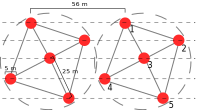
\includegraphics[width=0.8 \columnwidth]{lidar2img/fig/lola_shots.pdf}
	\caption{Two LOLA shots, part of a track. Each shot provides five
		distance measurements in a cross pattern. Shots are 56 m
		apart, and each laser beam reflects off a five meter diameter spot.}
	\label{fig:lolashots}
\end{figure}

The laser data is acquired from the Lunar Orbiter Laser Altimeter (LOLA), an instrument of the
Lunar Reconaissance Orbiter (LRO). The LOLA splits a laser into five parts to take five distance
measurements to the lunar surface, arranged in a cross shape. Each set of five measurements
is called a \emph{shot}. Each of the five laser beams
illuminates a 5 m diamter spot on the moon's surface (see Figure \ref{fig:lolashots}).

The LRO flies above the surface of the moon in a polar orbit, taking LOLA shots directly beneath
it as it moves.
Successive shots are approximately 56 m apart, and each sequence of shots from the same
orbit forms a \emph{track}. Figure \ref{fig:elevation} shows the elevation profile
of a crater as measured by two LOLA tracks.


\subsubsection{Aligning LIDAR to Images}

The data has two main sources of error: uncertainty in the position of the Apollo spacecraft's
position, and uncertainty in the position of the LRO when the LOLA shots were taken.
As Apollo 15 launched in 1971, 38 years
before the LRO, the Apollo images are subject to much larger position errors.

Uncertainty in Apollo 15's position affects the image's pose relative to all of the tracks, while
error in the LRO's position occurs on a per-track basis. We account for each of these
error sources separately, both using the Guass-Newton method. However, before we can align
the two data sources, we form a \emph{synthesized image} from the LOLA tracks that
can be easily compared to the Apollo image.

% image with tracks 100 and 113 in 24n26n2e4e_updated, Hadley C and Rima Hadley

{\bf Forming Synthesized Images}

\begin{figure}
	\centering
	\subfloat[LOLA Elevation Profile]{
	\includegraphics[width=0.8\columnwidth]{lidar2img/fig/hadley_elevation.pdf}
	\label{fig:elevation}}\\
	\subfloat[Before Coregistration]{
	\includegraphics[width=0.5\columnwidth]{lidar2img/fig/hadley_c_original.png}
	\label{fig:hadleyoriginal}}
	\subfloat[After Coregistration]{
	\includegraphics[width=0.5\columnwidth]{lidar2img/fig/hadley_c_adjusted.png}
	\label{fig:hadleyadjusted}}
	\caption{Two LOLA tracks that pass through the crater Hadley C and Rima Hadley are
		shown. \subref{fig:elevation} shows the LOLA tracks' elevation profiles.
		\subref{fig:hadleyoriginal} shows the tracks' estimated reflectance (the synthetic
		image) against an Apollo 15 image with the original alignment.
		\subref{fig:hadleyadjusted} shows the synthetic image and the Apollo 15 image after
		coregistration. The LOLA tracks are delineated by two bright lines, and the synthetic
		image is shown as the color between the lines.}
	\label{fig:problem}
\end{figure}

To align the LOLA tracks to the Apollo images, we estimate the lunar reflectance $r$ for each LOLA
shot to form a \emph{synthesized image}. The reflectance is a function of the angle of incidence
of light, which depends on the angle to the sun and the surface normal. The surface normal
is computed by adding the normals from each available triangle in the LOLA shot (see Figure \ref{fig:lolashots})
and normalizing the result. Some triangles' normals may not be available since LOLA does not always
succesfully return five surface readings.

Given the surface normal and the vector from the surface to the sun, we compute the expected reflectance with
the photometric equation presented in by McEwen. These estimated shot reflectances form
a synthetic image, which we expect to match the actual images taken during the Apollo mission.

The actual surface luminence seen in an image is given by the product of the reflectance and a constant factor, % TODO: is luminence right word?
$\alpha r$. The value of $\alpha$ depends on two factors: the parameters of the camera that took the image,
and the properties of the reflecting surface. The refletance properties of the lunar surface vary, particularly
between the flat, low-lying maria and the highlands. However, they are locally consistent.

Given a set of tracks, an image, and a transformation from track coordinates to image coordinates, we estimate the scaling factor $\alpha$.
Let $p$ be the list of all LOLA shots' transformed image coordinates, where $p_i^x$ and $p_i^y$ are the $x$ and $y$
coordinates of LOLA shot $i$ transformed by a matrix $M$, let $r$ be a list of all LOLA shots' estimated reflectances, and let $I$ be an image.
Then we compute the scaling
factor as the value which makes the average value of the actual image equal the 
average value of the synthetic image, $\alpha = \left(\sum I(p_i^x, p_i^y)\right) / \left(\sum L_i^r\right)$.
So $\alpha$ is a function of $M$.

{\bf The Gauss Newton Algorithm}

Let $L$ be a list of LOLA shots, where $L_i^x$ and $L_i^y$ denote the initial image coordinates and
$L_i^r$ denotes the estimated reflectance. Our goal is to find 
$$\arg \min_M S(M) = \arg \min_M \sum_i r_i(M)^2\mbox{,}$$
where $r_i(M)$ is the error for a single LOLA shot's synthetic image given the transformation matrix $M$,
the $3 \times 3$ homography that minimizes the error between the synthetic and the observed images.
$$r_i(m) = I\left(M \left[\begin{array}{c}L_i^x\\ L_i^y\\ 1\end{array}\right]\right) - \alpha L_i^r\mbox{.}$$
The true error in the satellites' positions cannot be accounted for with a planar homography, since the
surface of the moon and the LRO's motion are both non-planar. However, we have found that planar
homographies are an effective approximation across limited areas.

Minimizing this objective function is a non-linear least squares problem. A common tool for solving
such problems is the Gauss-Newton algorithm, a variant of Newton's method which doesn't require
the computation of second derivatives.

In each step of the algorithm, we find a change $\Delta$ to the parameters $\beta$ (the entries of $M$ written as
a vector) such that the error decreases, where $\beta_{t+1} = \beta_t + \Delta$. As with Newton's method,
we choose $\beta_{t+1}$ to be the point where the second-order Taylor expansion of $S$ 
reaches zero.

The second-order Taylor expansion of $S$ is given by
$$S(\beta + \Delta) \approx S(\beta) + J_S(\beta) \Delta + \frac{1}{2}\Delta^T H_S(\beta) \Delta$$
where $J_S(\beta)$ and $H_S(\beta)$ are the Jacobian and Hessian with respect to $\beta$, respectively.
Since $S$ is a function of $r$ (the error vector), we can rewrite the Jacobian of $S$ as a function of $r$.

\begin{eqnarray*}
	J_S(\beta) &=& \left[ \begin{array}{ccc}\frac{dS}{d\beta_1} & \ldots & \frac{dS}{d\beta_9}\end{array}\right]\\
	&=& \left[ \begin{array}{ccc}\frac{d}{d\beta_1}\sum_i r_i^2 & \ldots & \frac{d}{d\beta_9}\sum_i r_i^2\end{array}\right]\\
	&=& 2 \left[ \begin{array}{ccc}\sum_ir_i \frac{dr_i}{d\beta_1} & \ldots & \sum_i r_i \frac{dr_i}{d\beta_9}\end{array}\right]\\
	&=& 2 \left[ \begin{array}{ccc}r_1 & \cdots & r_n \end{array} \right]\left[
		\begin{array}{ccc}
		\frac{dr_1}{d\beta_1} & \ldots & \frac{dr_1}{d\beta_9}\\
		\vdots & \vdots & \vdots\\
		\frac{dr_n}{d\beta_1} & \ldots & \frac{dr_n}{d\beta_9}
		\end{array}\right]\\
	&=& 2 r^T J_r(\beta)
\end{eqnarray*}

\noindent Likewise, we can write the Hessian of $S$ as a function of $J_r(\beta)$.

\begin{eqnarray*}
	H_S(\beta) &=& \frac{d}{d\beta} \frac{dS}{d\beta}\\
	&=& \frac{d}{d\beta} 2 r^T J_r(\beta)\\
	&=& 2 \left(\left(\frac{dr}{d\beta}\right)^T J_r(\beta) + r^T \frac{d}{d\beta}J_r(\beta)\right)\\
	&=& 2 \left(J_r(\beta)^T J_r(\beta) + r^T \frac{d}{d\beta}J_r(\beta)\right)\\
	&\approx& 2 J_r(\beta)^T J_r(\beta)
\end{eqnarray*}

\noindent We approximate $H_S(\beta)$ with the simplifying assumptation that the error $r$ is low.

Now, we can rewrite the second-order Taylor approximation in terms of $J_r(\beta)$.
\begin{eqnarray*}
	S(\beta + \Delta) &\approx& S(\beta) + J_S(\beta) \Delta + \frac{1}{2}\Delta^T H_S(\beta) \Delta\\
	&\approx& S(\beta) + 2 r^T J_r(\beta) \Delta + \Delta^T J_r(\beta)^T J_r(\beta) \Delta\\
\end{eqnarray*}
\noindent The minimum occurs when the derivative of $S$ with respect to $\Delta$ is zero. We find this point based
on the second order-approximation.
\begin{eqnarray*}
0 &=& \frac{d}{d\Delta} S(\beta + \Delta)\\
  &\approx& 2 r^T J_r(\beta) + 2 \Delta^T J_r(\beta)^T J_r(\beta)\\
  -r^T J_r(\beta) &=& \Delta^T J_r(\beta)^T J_r(\beta)\\
  -\left(J_r(\beta)^T r\right)^T &=& \left(\left(J_r(\beta)^T J_r(\beta)\right)^T \Delta\right)^T\\
  -J_r(\beta)^T r &=& J_r(\beta)^T J_r(\beta) \Delta\\
\end{eqnarray*}
We solve this system of linear equations for $\Delta$ with an application of singular value decomposition.

Then, we continue taking steps with new $\delta$ until the error doesn't decrease. The full Gauss-Newton
algorithm is shown in Algorithm \ref{alg:gaussnewton}.

\begin{algorithm}
	\begin{algorithmic}
		\STATE $err_{old} = \infty$
		\LOOP
		\STATE $\forall i \in \{1,..,|L|\}~\left[\begin{array}{c}p_i^x\\p_i^y\\1\end{array}\right] =
				M \left[\begin{array}{c}L_i^x\\L_i^y\\1\end{array}\right]$
		\STATE $\alpha = \left(\sum I(p_i^x, p_i^y)\right) / \left(\sum L_i^r\right)$
		\STATE $\forall i \in \{1,..,|L|\}~E_i = I(p_i^x, p_i^y) - \alpha L_i^r$
		\STATE $err = \sum_i E_i^2$
		\IF{$err \ge err_{old}$}
			\RETURN $M_{prev}$
		\ENDIF
		\STATE $err_{old} = err$
		\STATE $J = \left[\begin{array}{cccccc}
			\frac{dI(p_1^x, p_1^y)}{dM_{1,1}}&\frac{dI(p_1^x, p_1^y)}{dM_{1,2}}&\frac{dI(p_1^x, p_1^y)}{dM_{1,3}}&\frac{dI(p_1^x, p_1^y)}{dM_{2,1}}&\frac{dI(p_1^x, p_1^y)}{dM_{2,2}}&\frac{dI(p_1^x, p_1^y)}{dM_{2,3}}\\
			\vdots&\vdots&\vdots&\vdots&\vdots&\vdots\\
			\frac{dI(p_n^x, p_n^y)}{dM_{1,1}}&\frac{dI(p_n^x, p_n^y)}{dM_{1,2}}&\frac{dI(p_n^x, p_n^y)}{dM_{1,3}}&\frac{dI(p_n^x, p_n^y)}{dM_{2,1}}&\frac{dI(p_n^x, p_n^y)}{dM_{2,2}}&\frac{dI(p_n^x, p_n^y)}{dM_{2,3}}\\
			\end{array}\right]$
		\STATE $D = \left(J^T J\right)^{-1} J^T E$
		\STATE $\Delta = \left[\begin{array}{ccc}
				D_1&D_2&D_3\\D_4&D_5&D_6\\0&0&1
			\end{array}\right]$
		\STATE $M_{prev} = M$
		\STATE $M = M + \Delta$
		\ENDLOOP
	\end{algorithmic}
	\caption{$\texttt{gauss\_newton}(L, I, M)$: Aligns a set of LOLA shots $L$ to an image $I$,
		given an initial transformation matrix $M$.}
	\label{alg:gaussnewton}
\end{algorithm}

%Gauss-Newton is a modification of Newton's method, designed to solve non-linear least squares problems
%without the need to compute second derivatives. Here, we attempt to minimize the square of the error between
%the synthetic image generated from LIDAR data and the actual image taken by Apollo 15. The Gauss-Newton
%algorithm as applied to this domain is outlined in Algorithm \ref{alg:gaussnewton}. It takes as inputs
%a list of LOLA shots, an Apollo image, along with an initial guess for the transformation matrix
%from LOLA shot coordinates to image coordinates. The Gauss-Newton algorithm refines this
%initial guess and returns an improved transformation matrix that reduces the error.


{\bf Search Over the Image Pyramid}

The Gauss-Newton algorithm, like Newton's method, is highly susceptible to local minima.
In our problem, the LOLA tracks begin highly misaligned, and a naive application of Gauss-Newton
will converge to nearby local minima rather than the global minima.

To prevent this, we first search
on downsampled, lower-resolution layers of the image pyramid (see Fig. \ref{fig:pyramid}).
By downsampling we find only a coarse alignment, but the lower resolution image allows us to
avoid local minima and coregister the tracks in the presence of large initial errors.

Once a coarse alignment is found, we align the LOLA tracks on progressively higher resolution
layers of the image pyramid using Algorithm \ref{alg:coregister}. Note that we must scale
the translational component of the transformation matrix between layers of the image
pyramid to account for the changed image coordinate system.

\begin{figure}
	\includegraphics[width=0.235\columnwidth]{lidar2img/fig/hadley_rille_8.png}
	\includegraphics[width=0.235\columnwidth]{lidar2img/fig/hadley_rille_4.png}
	\includegraphics[width=0.235\columnwidth]{lidar2img/fig/hadley_rille_2.png}
	\includegraphics[width=0.235\columnwidth]{lidar2img/fig/hadley_rille_1.png}
	\caption{Hadley Rille, as seen in multiple layers of the image pyramid. From left to right,
	downscaled by factors of 8, 4, 2, and 1.}
	\label{fig:pyramid}
\end{figure}

\begin{algorithm}
	\begin{algorithmic}
		\STATE $P = \texttt{image\_pyramid}(I, n)$
		\STATE $T_0 = \left[\begin{array}{ccc}1/2^n&0&0\\0&1/2^n&0\\0&0&1\end{array}\right]$
		\STATE $G = \texttt{gauss\_newton}(L, P_{n}, T_0)$
		\STATE $\forall~i\in\{1,\ldots,|T|\}~M_i = G$
		\FOR{$i$ from $n-1$ to $0$}
			\FOR{$j \in \{1,..,|T|\}$}
			\STATE $M_j = \left[\begin{array}{ccc}2&0&0\\0&2&0\\0&0&1\end{array}\right] M_j
				\left[\begin{array}{ccc}0.5&0&0\\0&0.5&0\\0&0&1\end{array}\right]$
			\STATE $M_j = \texttt{gauss\_newton}(L, P_{i}, M_j)$
			\ENDFOR
		\ENDFOR
		\RETURN $M$
	\end{algorithmic}
	\caption{$\texttt{coregister}(L, I)$: Given a list of LOLA tracks $L$ and an image $I$,
		return a list of transformations from track coordinates to image coordinates.}
	\label{alg:coregister}
\end{algorithm}

{\bf Computing the Jacobian}

Recall that the Gauss-Newton algorithm requires us to compute the Jacobian $J_r(\beta)$ of the error
with respect to the parameters of the transformation matrix. We skipped over this
previously, but now we discuss this in detail.

We aim to find the homography $H$ from track coordinates $(x, y)$ to image coordinates $(x', y')$.

\begin{eqnarray*}
\left[\begin{array}{ccc}
H_{11} & H_{12} & H_{13}\\
H_{21} & H_{22} & H_{23}\\
H_{31} & H_{32} & H_{33}
\end{array}\right]
\left[\begin{array}{c}x\\y\\1\end{array}\right] &=&
\left[\begin{array}{c}wx'\\wy'\\w\end{array}\right]\\
\left[\begin{array}{c}
H_{11}x + H_{12}y + H_{13}\\
H_{21}x + H_{22}y + H_{23}\\
H_{31}x + H_{32}y + H_{33}
\end{array}\right]
&=& \left[\begin{array}{c}wx'\\wy'\\w\end{array}\right]
\end{eqnarray*}

\begin{eqnarray*}
x' &=& \frac{H_{11}x + H_{12}y + H_{13}}{H_{31}x + H_{32}y + H_{33}}\\
y' &=& \frac{H_{21}x + H_{22}y + H_{23}}{H_{31}x + H_{32}y + H_{33}}\\
\end{eqnarray*}

For the Gauss-Newton algorithm, we require the partial derivatives of the image
with respect to each entry of the homography. For the first two rows of $H$, we
compute this by taking a finite difference with three points on the image, either
over a row in the image (for the first row of the homography) or over a column 
(for the second row). We use the finite difference with six points.

\begin{eqnarray*}
	\Delta I_x(x', y') &=& -\frac{1}{60}I(x'-3, y) + \frac{3}{20}I(x'-2, y') - \frac{3}{4} I(x'-1, y) +\\
			&& \frac{3}{4} I(x'+1, y) -\frac{3}{20}I(x'+2, y') + \frac{1}{60}I(x'+3, y)
\end{eqnarray*}

Once we find the change in the horizontal direction of the image, we find the change in the entries of $H$ with induces
a change of a single pixel in the image coordinates.

\begin{eqnarray*}
	\frac{(H_{11} + \Delta_{H_{11}}) x + H_{12}y + H_{13}}{H_{31}x + H_{32}y + H_{33}} - \frac{H_{11}x + H_{12}y + H_{13}}{H_{31}x + H_{32}y + H_{33}} &=& 1\\
	H_{31}x + H_{32}y + H_{33} &=& \Delta_{H_{11}} x\\
	\frac{H_{31}x + H_{32}y + H_{33}}{x} &=& \Delta_{H_{11}}\\
	\frac{H_{31}x + H_{32}y + H_{33}}{y} &=& \Delta_{H_{12}}\\
	H_{31}x + H_{32}y + H_{33} &=& \Delta_{H_{13}}
\end{eqnarray*}

Then we can approximate the partial derivatives as

$$\frac{dI}{dH_{11}} = \frac{\Delta I_x(x', y')}{\Delta H_{11}}, 
\frac{dI}{dH_{12}} = \frac{\Delta I_x(x', y')}{\Delta H_{12}}, 
\frac{dI}{dH_{13}} = \frac{\Delta I_x(x', y')}{\Delta H_{13}}$$

The equations are the same for the second row of $H$, except we take a finite
difference in the vertical direction instead:

$$\frac{dI}{dH_{21}} = \frac{\Delta I_y(x', y')}{\Delta H_{21}}, 
\frac{dI}{dH_{22}} = \frac{\Delta I_y(x', y')}{\Delta H_{22}}, 
\frac{dI}{dH_{23}} = \frac{\Delta I_y(x', y')}{\Delta H_{23}}$$

The third row of $H$ determines the scaling factor, which will multiply both
$x$ and $y$ by the same amount. If $x'> y'$, we find the change in $H$ which
brings us to the next pixel in the $x$ direction, if $y > x$ we find the change
to bring us to the next pixel in the $y$ direction. We interpolate between
neighboring pixels for non-integral image coordinates.

Let $m = \frac{y'}{x'}$. If $m \le 1$, we sample find the divided difference using pixels
with an even vertical offset. 

\begin{eqnarray*}
	\Delta I(x', y') &=& -\frac{1}{60}I(x'-3, y-3m) + \frac{3}{20}I(x'-2, y'-2m) - \frac{3}{4} I(x'-1, y-m) +\\
			&& \frac{3}{4} I(x'+1, y+m) -\frac{3}{20}I(x'+2, y'+2m) + \frac{1}{60}I(x'+3, y+3m)
\end{eqnarray*}

Likewise, if $m \ge 1$, we find the divided difference from pixels with a horizontal offset.

\begin{eqnarray*}
	\Delta I(x', y') &=& -\frac{1}{60}I(x'-\frac{3}{m}, y-3) + \frac{3}{20}I(x'-\frac{2}{m}, y'-2) - \frac{3}{4} I(x'-\frac{1}{m}, y-1) +\\
			&& \frac{3}{4} I(x'+\frac{1}{m}, y+1) -\frac{3}{20}I(x'+\frac{2}{m}, y'+2) + \frac{1}{60}I(x'+\frac{3}{m}, y+3)
\end{eqnarray*}

Next, we once again find the changes in $H$ which produce this $x$ or $y$ offset. First, if it is an $x$ offset:

$$\frac{H_{11} x + H_{12}y + H_{13}}{(H_{31} + \Delta H_{31})x + H_{32}y + H_{33}} - \frac{H_{11}x + H_{12}y + H_{13}}{H_{31}x + H_{32}y + H_{33}} = 1$$
$$\frac{H_{11} x + H_{12}y + H_{13}}{(H_{31} + \Delta H_{31})x + H_{32}y + H_{33}} = 1 + x'$$
$$H_{11} x + H_{12}y + H_{13} - (H_{32}y + H_{33})(1 + x') = (1 + x')\left(H_{31} + \Delta H_{31}\right)x$$
$$\frac{1}{x}\left(\frac{H_{11} x + H_{12}y + H_{13}}{(1+x')}- H_{32}y - H_{33}\right) - H_{31} = \Delta H_{31}$$
$$\frac{1}{y}\left(\frac{H_{11} x + H_{12}y + H_{13}}{(1+x')}- H_{31}x - H_{33}\right) - H_{32} = \Delta H_{32}$$
$$\frac{H_{11} x + H_{12}y + H_{13}}{(1+x')}- H_{31}x - H_{32}y - H_{33} = \Delta H_{33}$$

If it is a $y$ offset ($y' > x'$), the results are the same, except the entries from the first row of $H$ are replaced with
entries from the second row. Furthermore, $x'$ becomes $y'$. Then, once again, we find the derivatives.

$$\frac{dI}{dH_{31}} = \frac{\Delta I_y(x', y')}{\Delta H_{31}}, 
\frac{dI}{dH_{32}} = \frac{\Delta I_y(x', y')}{\Delta H_{32}}, 
\frac{dI}{dH_{33}} = \frac{\Delta I_y(x', y')}{\Delta H_{33}}$$

Now we are able to generate the Jacobian $J_r(\beta)$.


\subsubsection{Selected Results}

Next, we show selected results with Gauss-Newton on an image pyramid aligning
LOLA tracks to Apollo-15 images. Figures \ref{fig:monshadley} and \ref{fig:aratus}
show the position of the LOLA tracks on an Apollo image both before and after
finding a transformation. The red lines indicate the tracks, and the color
between them indicates the expected luminence of the moon based on the surface
normal, sun position and camera position. The intial error in both cases is large,
as seen by the large mismatch between the color of the LOLA track and the
background image.

After Gauss-Newton on the image pyramid is applied, a successful transformation is found.
The expected luminence closely matches the actual luminence.

\begin{figure}
	\centering
	\subfloat[Before Coregistration]{
	\includegraphics[width=0.5\columnwidth]{lidar2img/fig/mons_hadley_original_c.png}
	\label{fig:monshadleyoriginal}}
	\subfloat[After Coregistration]{
	\includegraphics[width=0.5\columnwidth]{lidar2img/fig/mons_hadley_adjusted_c.png}
	\label{fig:monshadleyadjusted}}
	\caption{LOLA tracks passing through the western part of Mons Hadley are shown
		\subref{fig:monshadleyoriginal} before coregistration, and
		\subref{fig:monshadleyadjusted} after coregistration. Note how after
		coregistration, the synthetic image matches the actual image much more closely.}
	\label{fig:monshadley}
\end{figure}

\begin{figure}
	\centering
	\subfloat[Before Coregistration]{
	\includegraphics[width=0.5\columnwidth]{lidar2img/fig/aratus_original.png}
	\label{fig:aratusoriginal}}
	\subfloat[After Coregistration]{
	\includegraphics[width=0.5\columnwidth]{lidar2img/fig/aratus_adjusted.png}
	\label{fig:aratusadjusted}}
	\caption{LOLA tracks over Aratus crater
		\subref{fig:monshadleyoriginal} before coregistration, and
		\subref{fig:monshadleyadjusted} after coregistration. The sides of the
		crater form distinctive visual features.}
	\label{fig:aratus}
\end{figure}

% TODO: numeric error
Although our algorithm allows us to find general planar homographies from the track coordinates to
image coordinates, in practice the transformations that are found are affine transformations. They
have a large translational component and a slight rotational component.


\subsubsection{Conclusion}

We have presented the algorithm that aligns oribital LIDAR data to image data
in the presence of substantial position errors implemented by the {\texttt{lidar2img}} program.
The algorithm applies Gauss-Newton
on an image pyramid to avoid local minima. We have demonstrated the algorithm's
success on lunar data, and successfully coregistered LIDAR and image data of the moon. 




\section{Structure from Motion(SFM) in sfm\_ processing module}
\label{sec:sfm}
\subsection{Files:}
\begin{itemize}
	\item{sfm\_test.cpp} - main function for SFM Processing
	\item{SFM.h} - declaration of SFM class
	\item{SFM.cpp} - definition of SFM class
	\item{PoseEstimation.h} - declaration of PoseEstimation class
	\item{PoseEstimation.cpp} - definition of PoseEstimation class
	\item{FeatureExtraction.h} - declaration of FeatureExtraction class
	\item{FeatureExtraction.cpp} - definition of FeatureExtraction class
	\item{sfm\_config.txt} - configuration file for main program
\end{itemize}


\subsection{How to install sfm:}
\begin{enumerate}
	\item{Install Prerequisites} - Install OpenCV 2.3.1, PCL 1.5, lapack, cmake, gfortran
	\item{Install SFM} - inside sfm processing directory type: cmake .
	\item{Build sfm\_test} - inside sfm processing directory type: make
	\item{Run Examples} - ./sfm\_test testConfig.txt testImageList.txt results
\end{enumerate}

\subsection{Configuration Parameters}
If the configuration file is not specified, the program will run with a set of default parameters.
\begin{itemize}
	\item{\textsc{depthInfo}} - 0 (No Depth), 2 (Kinect Depth), 3 (Stereo Point Clouds)
	\item{\textsc{pointCloudFilename}} - file containing filenames for all point cloud files
	\item{\textsc{kinectDepthFilename}} - file containing list of kinect depth filenames
	\item{\textsc{minMatches}} - minimum number of matches in order to do pose estimation
	\item{\textsc{detThresh}} - small threshold for determinant of R in order to do SVD
	\item{\textsc{featureMethod}} - 0 (SURF), 1 (ORB), 2 (SIFT)
	\item{\textsc{poseEstimationType}} - 0 (Pairs of frames for Pose Estimation), 1 (SBA)
	\item{\textsc{nndrRatio}} - ratio for determining good matches
	\item{\textsc{numNN}} - number of nearest neighbors to save for each key point
	\item{\textsc{zDist}} - maximum distance between z coordinates for good matches
	\item{\textsc{xDist}} - maximum distance between x coordinates for good matches
	\item{\textsc{yDist}} - maximum distance between y coordinates for good matches
	\item{\textsc{nbMatches}} - minimum number of matches for homography
	\item{\textsc{homographyMethod}} - 0 (Default OpenCV Method), 4 (Least Median Method), 8 (RANSAC Method)
	\item{\textsc{flannCheck}} - number of elements to visit in NN search
	\item{\textsc{ransacPixels}} - maximum number of pixels the match can be from the epipolar line
	\item{\textsc{ransacAccuracy}} - accuracy of homography before stopping iterations
	\item{\textsc{tileWidth}} - width of each tile in image
	\item{\textsc{tileHeight}} - height of each tile in image
	\item{\textsc{xOverlap}} - amount of overlap in the x direction between consecutive tiles
	\item{\textsc{yOverlap}} - amount of overlap in the y direction between consecutive tiles
	\item{\textsc{tileScaleX}} - scale from reference tile to matching tile in the x direction
	\item{\textsc{tileScaleY}} - scale from reference tile to matching tile in the y direction
	\item{\textsc{pointProjFilename}} - file where point projections are saved for later use by SBA
	\item{\textsc{weightedPortion}} - weights this portion of the image to the bottom of the image (work in progress \ldots)
\end{itemize}


%=======
%\section{Installation of SFM}

%This is complete installation procedure for Mac OS X.

%\begin{lstlisting}
%- install prerequisites
%1) install Macport (http://www.macports.org/install.php) 
%2) install dependencies (http://pointclouds.org/downloads/macosx.html)
%3) install PCL (http://pointclouds.org/downloads/macosx.html)
%4) sudo port install opencv
%5) sudo port install cmake
%6) install gfortran (http://gcc.gnu.org/wiki/GFortranBinaries)
%7) install lapack(http://gcc.gnu.org/testing/testing-lapack.html)
%7.1) download lapack.tgz and unzip it
%7.2) rename make.inc.example to make.inc in the root directory of lapack 
%7.3) make blaslib && make
%8) install sba (http://www.ics.forth.gr/~lourakis/sba/) 
%8.1) edit demo/CMakeLists.txt

%# CMake file for sba's demo program

%INCLUDE_DIRECTORIES(..)
%LINK_DIRECTORIES(.. ${LAPACKBLAS_DIR})

%ADD_EXECUTABLE(eucsbademo eucsbademo.c imgproj.c readparams.c eucsbademo.h readparams.h)
%# libraries the demo depends on
%IF(HAVE_F2C)
%  TARGET_LINK_LIBRARIES(eucsbademo sba ${LAPACK_LIB} ${BLAS_LIB} ${F2C_LIB})
%ELSE(HAVE_F2C)
%  TARGET_LINK_LIBRARIES(eucsbademo sba ${LAPACK_LIB})
%ENDIF(HAVE_F2C)

%# make sure that the library is built before the demo
%ADD_DEPENDENCIES(eucsbademo sba)

%8.2) mkdir build && cd build
%8.3) ccmake ..
%8.3.1) turn HAVE_F2C OFF
%8.3.2) LAPACK_LIB = -framework vecLib
%8.4) make
%8.5) set PATH for the libsba.a

%For beginner, check opt/local if you install them with "sudo port install." Otherwise, usr/local

%- Initialize SFM
%1) svn co https://babelfish.arc.nasa.gov/svn/stereopipeline/sandbox/sfm/
%2) cd sfm
%3) mkdir build
%4) cd build
%5) cmake .. (here is big double dots)
%6) make -j2 && make install

%- Configure SFM
%1) cd sfm\build
%2) ccmake ..
%[Press 'c' to configure]
%[Select option 'BUILD_TESTS']
%[Press 'c' to reconfigure]
%[Press 'g' to generate]

%# Test SFM
%1) cd sfm/build
%2) make test
%3) view the file in sfm/build/Testing/Tempory/LastTest.log

%# Run SFM with an Example
%1) cd sfm/examples
%2) scp <username>@<machinename>:/irg/data/kinect/<directory> .
%3) cd <directory>
%4) cp ../sfm_config_example.txt sfm_config.txt
%5) cp ../camera_calibration_example.txt camera_calibration.txt
%6) open sfm_config.txt to change the value of inputDataName by <directory>
%7) sfm
%8) pc_vis <directory>.txt

%for example <directory>=2011_1202_bldg_269_2, <machinename>=pesto
%1) cd sfm/examples
%2) scp <username>@pesto:/irg/data/kinect/2011_1202_bldg_269_2 .
%3) cd 2011_1202_bldg_269_2
%4) cp ../sfm_config_example.txt sfm_config.txt
%5) cp ../camera_calibration_example.txt camera_calibration.txt
%6) open sfm_config.txt: inputDataName 2011_1202_bldg_269_2
%7) sfm
%8) pc_vis 2011_1202_bldg_269_2.txt

%# troubleshooting
%If any problem to link dependencies,
%Download PCL sources from http://pointclouds.org/downloads/ 
%- compile and install PCL
%1) cd PCL-<ver>-Source
%2) cmake .
%3) make
%4) make install

%Add the following to ~/.bash_profile file
%export DYLD_FALLBACK_LIBRARY_PATH=/usr/local/lib:/usr/lib
%\end{lstlisting}

%\end{document}

\section{Stereo Disparity Maps in stereo\_ processing module}
\label{sec:stereo}

\subsection{Files:}

\begin{itemize}
\item{tests/CvStereoBMTest.cpp - main function for stereo using the block matching algorithm}
\item{tests/stereo\_settingsBM.txt - settings file for the block matching test}
\item{tests/CvStereoSGBMTest.cpp - main function for stereo using the semiglobal block matching algorithm (Hirschmuller)}
\item{tests/stereo\_settingsSGBM.txt - settings file for the semiglobal block matching test}
\item{tests/stereo\_calibration.txt - calibration file for stereo tests}
\item{CvStereoBMProcessor.h - declaration of stereo block matching class}
\item{CvStereoBMProcessor.cpp - definition of stereo block matching class}
\item{CvStereoSGBMProcessor.h - declaration of stereo semiglobal block matching class}
\item{CvStereoSGBMProcessor.cpp - definition of stereo semiglobal block matching class}
\end{itemize}


\subsection{How to install:}
\begin{enumerate}
	\item{Install Prerequisites - Install OpenCV 2.3, cmake} 
	\item{Install Stereo - inside stereo\_processing/tests directory type: "cmake ." } 
	\item{Build Stereo tests - inside stereo\_processing/tests directory type: "make" }  
	\item{Run Examples} 
\end{enumerate}

\subsection{How to run:}
\begin{enumerate}
   \item{./bm\_stereo\_test -a left.pgm -b right.pgm}
   \item{./sgbm\_stereo\_test -a left.pgm -b right.pgm}
\end{enumerate}

\subsection{Block Matching Configuration Parameters}
If the configuration file is not specified, the program will run with a set of default parameters.
\begin{itemize}
	\item{\textsc{PRE\_FILTER\_SIZE} - size of the preprocessing filter}
	\item{\textsc{PRE\_FILTER\_CAP} - parameter for OpenCV stereoBM}
	\item{\textsc{SAD\_WINDOW\_SIZE} - size of the SAD Window (must be odd)}
   \item{\textsc{MIN\_DISPARITY} - minimum possible disparity value}
   \item{\textsc{NUMBER\_OF\_DISPARITIES} - maximum possible disparity minus the minimum (must be a multiple of 16)} 
   \item{\textsc{TEXTURE\_THRESHOLD} - minimum texture value for a pixel to be reliable}
   \item{\textsc{UNIQUENESS\_RATIO} - margin in percentage by which a match should score higher than the second best to be considered a match}
   \item{\textsc{NEED\_RECTIFICATION} - set to YES if the images need to be rectified, NO otherwise}
   \item{\textsc{DOWNSAMPLE\_FACTOR} - factor by which to scale the images prior to processing}
   \item{\textsc{CALIBRATION\_FILENAME} - filename where the calibration information is stored}
   \item{\textsc{TILE\_WIDTH} - width of tile for processing by tiles, set to -1 for no tiling}
   \item{\textsc{TILE\_HEIGHT} - height of tile for processing by tiles, set to -1 for no tiling}
\end{itemize}

\subsection{Semiglobal Block Matching Configuration Parameters}
If the configuration file is not specified, the program will run with a set of default parameters.
\begin{itemize}
	\item{\textsc{PRE\_FILTER\_CAP }} - truncates the x derivates to [-preFilterCap,preFilterCap]
	\item{\textsc{SAD\_WINDOW\_SIZE} - size of the SAD Window (must be odd)}
	\item{\textsc{P1} - penalty on the disparity change by 1 (OpenCV suggests starting at about 8*imageChannels*sadWindowSize*sadWindowSize)}
	\item{\textsc{P1} - penalty on the disparity change by more than 1 (OpenCV suggests starting at about 32*imageChannels*sadWindowSize*sadWindowSize)}
   \item{\textsc{MIN\_DISPARITY} - minimum possible disparity value}
   \item{\textsc{NUMBER\_OF\_DISPARITIES} - maximum possible disparity minus the minimum (must be a multiple of 16)} 
   \item{\textsc{UNIQUENESS\_RATIO} - margin in percentage by which a match should score higher than the second best to be considered a match}
   \item{\textsc{NEED\_RECTIFICATION} - set to YES if the images need to be rectified, NO otherwise}
   \item{\textsc{DOWNSAMPLE\_FACTOR} - factor by which to scale the images prior to processing}
   \item{\textsc{CALIBRATION\_FILENAME} - filename where the calibration information is stored}
   \item{\textsc{TILE\_WIDTH} - width of tile for processing by tiles, set to -1 for no tiling}
   \item{\textsc{TILE\_HEIGHT} - height of tile for processing by tiles, set to -1 for no tiling}
\end{itemize}



\section{Utilities in common module}
\label{sec:common}
The files in common are used for several different modules in the Alignment Toolkit.

\subsection{Files:}
\begin{itemize}
\item{pc\_vis.cpp} - point cloud viewer
\item{Tiling.h} - declaration of Tiling class
\item{Tiling.cpp} - definition of Tiling class
\item{pds\_read.h} - declaration of functions that read data from pds files
\item{pds\_read.cpp} - definition of functions that read data from pds files
\item{opencv\_pds.h} - declaration of functions to read pds images into OpenCV images
\item{opencv\_pds.cpp} - definition of functions to read pds images into OpenCV images
\item{tests/tilingTest.cpp} - test file for class
\item{tests/tileConfig.txt} - configuration file for tile test
\item{tests/testImageList.txt} - list of test images to run tilingTest on
\item{tests/test\_read.cpp} - test file for the opencv pds image reader

\end{itemize}

\subsection{How to install:}
\begin{enumerate}
	\item{Install Prerequisites} - OpenCV 2.3.1, PCL 1.5, cmake 
   \item{Install} pds tools from http://pds.nasa.gov/tools/pds-tools-package.shtml To install run batch\_make in /src. 
   \item{Set} environment variable OALROOT to the root of the pds tools install
	\item{Build} - cd common/tests and type cmake . and then make
\end{enumerate}

\subsection{How to run:}
\begin{itemize}
	\item{pc\_vis} - ./pc\_vis PC.txt
	\item{tilingTest} - ./tiling tileConfig testImageList
	\item{pdsReadTest} - ./pdsReadTest testImage.img
\end{itemize}
\subsubsection{Configuration Parameters}
If the configuration file is not specified, the program will run with a set of default parameters.
\begin{itemize}
	\item{\textsc{tileWidth}} - width of each tile
	\item{\textsc{tileHeight}} - height of each tile
	\item{\textsc{xOverlap}} - overlap of each tile in the x direction
	\item{\textsc{yOverlap}} - overlap of each tile in the y direction
\end{itemize}




\end{document}
